% This is text associated with the open textbook "Open Electromagnetics"
% See immediately below for author, date
% This work is licensed under the Creative Commons Attribution-ShareAlike 4.0 International License. (CC BY-SA 4.0) 
% To view a copy of the license, visit http://creativecommons.org/licenses/by-sa/4.0/

%ORB TITLE Solution of the Wave Equation for Magnetic Vector Potential
%ORB AUTHOR 0        # S.W. Ellingson, Virginia Tech (ellingson@vt.edu)
%ORB DATE 20191123   # yyyymmdd
%ORB ABSTRACT 

\label{m0196_Solution_of_the_Wave_Equation_for_Magnetic_Vector_Potential} % <-- Must match name of this file and module directory name.  Don't mess with this!
\index{magnetic vector potential|(}

The magnetic vector potential $\widetilde{\bf A}$ due to a current density $\widetilde{\bf J}$ is given by the following wave equation:
\index{wave equation!electromagnetic}
\index{wave equation!magnetic vector potential}
%
\begin{equation}
\nabla^2 \widetilde{\bf A}
-\gamma^2\widetilde{\bf A} 
= 
-\mu\widetilde{\bf J}
\label{m0196_ePDEA}
\end{equation}
%
where $\gamma$ is the \emph{propagation constant}, 
\index{propagation constant}
defined in the usual manner\footnote{Alternatively, $\gamma^2\triangleq -\omega^2\mu\epsilon_c$ accounting for the possibility of lossy media.}
%
\begin{equation}
\gamma^2\triangleq -\omega^2\mu\epsilon
\end{equation}
%
Equation~\ref{m0196_ePDEA} is a partial differential equation which is inhomogeneous (in the mathematical sense) and can be solved given appropriate boundary conditions.
In this section, we present the solution for arbitrary distributions of current in free space.

The strategy is to first identify a solution for a distribution of current that exists at a single point.  
This distribution is the \emph{current moment}.
\index{current moment}
An example of a current moment is shown in Figure~\ref{m0196_fCurrentMoment}.
%
\begin{figure}[b!] % <--- "[b!]" for first figure in section *only*; delete for 2nd and subsequent figures
\begin{center}
\pdftooltip{{  % note double braces
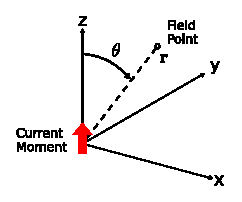
\includegraphics[width=2in]{modules/m0196_fCurrentMoment.eps} 
% https://commons.wikimedia.org/wiki/File:A_z-directed_current_moment_located_at_the_origin.svg
}}{An x-y-z Cartesian coordinate system with z vertical, x horizontal, and y into the page. For a field point labeled bold small r is an angle theta from the positive z axis. Thick arrow labeled "current moment" at the origin pointing up.}
\end{center}
\centerline{\scriptsize 
\copyright~\hyperref[m0196_fCurrentMoment_Credit]{C.\ Wang} 
\href{https://creativecommons.org/licenses/by-sa/4.0/}{CC BY-SA 4.0} 
} % \centerline 
\caption{
\label{m0196_fCurrentMoment}
An example of a current moment located at the origin.  In this case, $\hat{\bf l}=\hat{\bf z}$.
}
\end{figure}
%
A general expression for a current moment located at the origin is:
%
\begin{equation}
\widetilde{\bf J}({\bf r}) = \hat{\bf l}~\widetilde{I}~\Delta l~\delta({\bf r})
\label{m0196_eCM}
\end{equation}
%
where 
$\widetilde{I}$ has units of current (SI base units of A),
$\Delta l$ has units of length (SI base units of m),
$\hat{\bf l}$ is the direction of current flow,
and $\delta({\bf r})$ is the volumetric sampling function\footnote{Also a form of the \emph{Dirac delta function};
\index{Dirac delta function} 
see ``Additional Reading'' at the end of this section.}
\index{sampling function}
defined as follows:
%
\begin{flalign}
~ &\delta({\bf r}) \triangleq 0~~~ \mbox{for}~~~ {\bf r}\neq 0;~~~ \mbox{and} \label{m0196_eDelta1} \\
~ &\int_{\mathcal{V}}\delta({\bf r})~dv \triangleq 1             \label{m0196_eDelta2}
\end{flalign}
%
where
$\mathcal{V}$ is any volume which includes the origin (${\bf r}=0$).
It is evident from Equation~\ref{m0196_eDelta2} that $\delta({\bf r})$ has SI base units of m$^{-3}$; i.e., inverse volume.
Subsequently ${\bf J}({\bf r})$ has SI base units of A/m$^2$, indicating that it is a volume current density.\footnote{Remember, the density of a volume current is with respect to the \emph{area} through which it flows, therefore the units are A/m$^2$.}
-- as indicated by Equation~\ref{m0196_eDelta1} -- it exists only at the origin and nowhere else.
  
Substituting Equation~\ref{m0196_eCM} into Equation~\ref{m0196_ePDEA}, we obtain: 
%
\begin{equation}
\nabla^2 \widetilde{\bf A}
-\gamma^2\widetilde{\bf A} 
= 
-\mu\hat{\bf l}~\widetilde{I}~\Delta l~\delta({\bf r}) 
\label{m0196_ePDEAC}
\end{equation}
%
The general solution to this equation presuming homogeneous and time-invariant media (i.e., $\mu$ and $\epsilon$ constant with respect to space and time) is:
%
\begin{equation}
\widetilde{\bf A}({\bf r}) = \hat{\bf l}~\mu~\widetilde{I}~\Delta l~\frac{e^{\pm \gamma r}}{4\pi r}
\label{m0196_eA}
\end{equation}
% 
To confirm that this is a solution to Equation~\ref{m0196_ePDEAC}, substitute this expression into Equation~\ref{m0196_ePDEA} and observe that the equality holds.

Note that Equation~\ref{m0196_eA} indicates two solutions, corresponding to the signs of the exponent in the factor $e^{\pm \gamma r}$.
We can actually be a little more specific by applying some common-sense physics.
Recall that $\gamma$ in general may be expressed in terms of real and imaginary components as follows:
%
\begin{equation}
\gamma = \alpha + j\beta
\end{equation}
%
where $\alpha$ is a real-valued positive constant known as the \emph{attenuation constant}
\index{propagation constant!attenuation}
and $\beta$ is a real-valued positive constant known as the \emph{phase propagation constant}.
\index{propagation constant!phase}
%
Thus, we may rewrite Equation~\ref{m0196_eA} as follows:
%
\begin{equation}
\widetilde{\bf A}({\bf r}) = \hat{\bf l}~\mu~\widetilde{I}~\Delta l~\frac{ e^{\pm \alpha r} e^{\pm j\beta r} }{4\pi r} 
\label{m0196_eA2}
\end{equation}
%
Now consider the factor $e^{\pm \alpha r}/r$, which determines the dependence of magnitude on distance $r$.
If we choose the negative sign in the exponent, this factor decays exponentially with increasing distance from the origin, ultimately reaching zero at $r\rightarrow\infty$.
This is precisely the expected behavior, since we expect the magnitude of a radiated field to diminish with increasing distance from the source.
If on the other hand we choose the positive sign in the exponent, this factor increases to infinity as $r\rightarrow\infty$.
That outcome can be ruled out on physical grounds, since it implies the introduction of energy independently from the source.
The requirement that field magnitude diminishes to zero as distance from the source increases to infinity is known as the \emph{radiation condition}, 
\index{radiation condition}
and is essentially a boundary condition that applies at $r\rightarrow\infty$.
Invoking the radiation condition, Equation~\ref{m0196_eA} becomes:
%
\begin{equation}
\widetilde{\bf A}({\bf r}) = \hat{\bf l}~\mu~\widetilde{I}~\Delta l~\frac{e^{-\gamma r}}{4\pi r}
\label{m0196_eA3}
\end{equation}
%
In the loss-free ($\alpha=0$) case, we cannot rely on the radiation condition to constrain the sign of $\gamma$.  
However, in practical engineering work there is always some media loss; i.e., $\alpha$ might be negligible but is not quite zero.
Thus, we normally assume that the solution for lossless (including free space) conditions is given by Equation~\ref{m0196_eA3} with $\alpha=0$:
%
\begin{equation}
\widetilde{\bf A}({\bf r}) = \hat{\bf l}~\mu~\widetilde{I}~\Delta l~\frac{e^{-j \beta r}}{4\pi r}
\label{m0196_eA4}
\end{equation}

Now consider the factor $e^{-j \beta r}$ in Equation~\ref{m0196_eA4}.
This factor exclusively determines the dependence of the phase of $\widetilde{\bf A}({\bf r})$ with increasing distance $r$ from the source. 
In this case, we observe that surfaces of constant phase correspond to spherical shells which are concentric with the source.
Thus, $\widetilde{\bf A}({\bf r})$ is a spherical wave.

Let us now consider a slightly more complicated version of the problem in which the current moment is no longer located at the origin, but rather is located at ${\bf r}'$.  
This is illustrated in Figure~\ref{m0196_fCurrentMomentDisplaced}.
%
\begin{figure} % <--- "[b!]" for first figure in section *only*; delete for 2nd and subsequent figures
\begin{center}
\pdftooltip{{  % note double braces
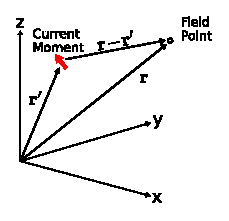
\includegraphics[width=2in]{modules/m0196_fCurrentMomentDisplaced.eps} 
% https://commons.wikimedia.org/wiki/File:Current_moment_displaced_from_the_origin.svg
}}{An x-y-z Cartesian coordinate system with z vertical, x horizontal, and y going into the page. Vector boldface small r points from origin to field point. Vector boldface small r prime points from origin to a point closer to the z axis. Distance between vectors is boldface small r minus boldface small r prime. Current moment positioned at small r prime and points in the negative x direction.
}
\end{center}
\centerline{\scriptsize 
\copyright~\hyperref[m0196_fCurrentMomentDisplaced_Credit]{C.\ Wang} 
\href{https://creativecommons.org/licenses/by-sa/4.0/}{CC BY-SA 4.0} 
} % \centerline 
\caption{
\label{m0196_fCurrentMomentDisplaced}
Current moment displaced from the origin.
}
\end{figure}
%
This current distribution can be expressed as follows:
%
\begin{equation}
\widetilde{\bf J}({\bf r}) = \hat{\bf l}~\widetilde{I}~\Delta l~\delta({\bf r}-{\bf r}')
%\label{m0196_eCM2}
\end{equation}
%
The solution in this case amounts to a straightforward modification of the existing solution.
To see this, note that $\widetilde{\bf A}$ depends only on $r$, and not at all on $\theta$ or $\phi$.  
In other words, $\widetilde{\bf A}$ depends only on the distance between the ``field point'' ${\bf r}$ at which we observe $\widetilde{\bf A}$, and the ``source point'' ${\bf r}'$ at which the current moment lies.
Thus we replace $r$ with this distance, which is $\left|{\bf r}-{\bf r}'\right|$. 
The solution becomes:
%
\begin{equation}
\widetilde{\bf A}({\bf r}) = \hat{\bf l}~\mu~\widetilde{I}~\Delta l~\frac{e^{-\gamma \left|{\bf r}-{\bf r}'\right|}}{4\pi \left|{\bf r}-{\bf r}'\right|}
\end{equation}

Continuing to generalize the solution, let us now consider a scenario consisting of a filament of current following a path $\mathcal{C}$ through space.  
This is illustrated in Figure~\ref{m0196_fCurrentFilament}.
%
\begin{figure} % <--- "[b!]" for first figure in section *only*; delete for 2nd and subsequent figures
\begin{center}
\pdftooltip{{  % note double braces
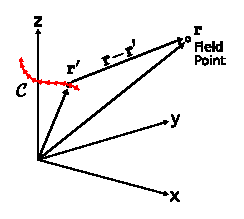
\includegraphics[width=2in]{modules/m0196_fCurrentFilament.eps} 
% https://commons.wikimedia.org/wiki/File:A_filament_of_current_lying_along_the_path_c.svg
}}{An x-y-z Cartesian coordinate system with z vertical, x horizontal, and y going into the page. Vector boldface small r points from origin to field point. Vector boldface small r prime points from origin a point closer to the z axis. Distance between vectors is boldface small r minus boldface small r prime. Current moment positioned at small r prime and points in the negative x direction following a curved path labeled capital C. 
}
\end{center}
\centerline{\scriptsize 
\copyright~\hyperref[m0196_fCurrentFilament_Credit]{C.\ Wang} 
\href{https://creativecommons.org/licenses/by-sa/4.0/}{CC BY-SA 4.0} 
} % \centerline
\caption{
\label{m0196_fCurrentFilament}
A filament of current lying along the path $\mathcal{C}$.  This current distribution may be interpreted as a collection of current moments lying along $\mathcal{C}$.
}
\end{figure}
%
Such a filament may be viewed as a collection of a large number $N$ of discrete current moments distributed along the path.  The contribution of the $n^{\mbox{th}}$ current moment, located at ${\bf r}_n$, to the total magnetic vector potential is:
%
\begin{equation}
\Delta \widetilde{\bf A}({\bf r};{\bf r}_n) = \hat{\bf l}({\bf r}_n)~\mu~\widetilde{I}({\bf r}_n)~\Delta l~\frac{e^{-\gamma \left|{\bf r}-{\bf r}_n\right|}}{4\pi \left|{\bf r}-{\bf r}_n\right|}
\end{equation}
%
Note that we are allowing both the current $\widetilde{I}$ and current direction $\hat{\bf l}$ to vary with position along $\mathcal{C}$.
Assuming the medium is linear, superposition applies. 
So we add these contributions to obtain the total magnetic vector potential:
 %
\begin{flalign}
\widetilde{\bf A}({\bf r}) &\approx \sum_{n=1}^{N} \Delta \widetilde{\bf A}({\bf r};{\bf r}_n) \\
                           &\approx \frac{\mu}{4\pi} ~\sum_{n=1}^N \hat{\bf l}({\bf r}_n)~\widetilde{I}({\bf r}_n) ~\frac{e^{-\gamma \left|{\bf r}-{\bf r}_n\right|}}{\left|{\bf r}-{\bf r}_n\right|}~\Delta l
\end{flalign}
%
Now letting $\Delta l\rightarrow 0$ so that we may replace $\Delta l$ with the differential length $dl$:
 %
\begin{equation}
\boxed{
\widetilde{\bf A}({\bf r}) = \frac{\mu}{4\pi}~\int_{\mathcal{C}} \hat{\bf l}({\bf r}')~\widetilde{I}({\bf r}')~\frac{e^{-\gamma \left|{\bf r}-{\bf r}'\right|}}{\left|{\bf r}-{\bf r}'\right|} ~dl
}
\label{m0196_eAL}
\end{equation}
%
where we have also replaced ${\bf r}_n$ with the original notation ${\bf r}'$ since we once again have a continuum (as opposed to a discrete set) of source locations.
%
%%%%%%%%%%%%%%%%%%%%%%%%%%%%%%%%%%%%%%%%%%%%%%%
%ORB HIGHLIGHT
\begin{mdframed}[backgroundcolor=yellow!20,nobreak=true] 
The magnetic vector potential corresponding to radiation from a line distribution of current is given by Equation~\ref{m0196_eAL}. 
\end{mdframed}
%%%%%%%%%%%%%%%%%%%%%%%%%%%%%%%%%%%%%%%%%%%%%%%

Given $\widetilde{\bf A}({\bf r})$, the magnetic and electric fields may be determined using the procedure developed in Section~\ref{m0195_Magnetic_Vector_Potential}.

%%%%%%%%%%%%%%%%%%%%%

{\bf Additional Reading:}
\begin{itemize}
\item ``\href{https://en.wikipedia.org/wiki/Magnetic_potential}{Magnetic potential}'' on Wikipedia.
\item ``\href{https://en.wikipedia.org/wiki/Dirac_delta_function}{Dirac delta function}'' on Wikipedia.
\end{itemize}

\index{magnetic vector potential|)}


